\documentclass{article}
\usepackage{helvet,palatino,geometry,graphicx,titlesec,wrapfig}
\sffamily
\title{PsySound3 User Manual \\ DRAFT}
\graphicspath{{./images/}}
\author{Sam Ferguson, Densil Cabrera, Emery Schubert and Farhan Rizwi}
\begin{document}

	\maketitle
	\tableofcontents
\section{Introduction}

PsySound3 is a program for analysing audio files. It's purpose is to facilitate research into areas of audio and acoustics that rely on mathematical models that are applied to digitally recorded sound files, and to simplify the process for obtaining features from an audio file. One of the main research areas that relies on these types of models is psychoacoustical modelling, which can be concerned with auditory features such as the  `roughness' and `loudness' of the sound. Another overlapping area is musical psychology, which can be concerned with features such as tempo and articulation. 

The program aims to do three things, 
\begin{itemize} 
	\item to use the existing body of work by researchers in this area;
	\item to be easy to use by students and researchers alike;
	\item to be flexible enough to allow easy extension and alteration for research purposes.
\end{itemize}

This manual seeks to explain how to use the program. 

\subsection{Warning}

\begin{center}
THE SOFTWARE IS PROVIDED ``AS IS'', WITHOUT WARRANTY OF ANY KIND, EXPRESS OR IMPLIED, INCLUDING BUT NOT LIMITED TO THE WARRANTIES OF MERCHANTABILITY, FITNESS FOR A PARTICULAR PURPOSE AND NONINFRINGEMENT. IN NO EVENT SHALL THE AUTHORS OR COPYRIGHT HOLDERS BE LIABLE FOR ANY CLAIM, DAMAGES OR OTHER LIABILITY, WHETHER IN AN ACTION OF CONTRACT, TORT OR OTHERWISE, ARISING FROM, OUT OF OR IN CONNECTION WITH THE SOFTWARE OR THE USE OR OTHER DEALINGS IN THE SOFTWARE.
\end{center}

To explain, we make a lot of effort to make sure that the algorithms supplied work as intended and can be calibrated accurately. However, many of the algorithms can be used in numerous ways, and testing against all possible uses is a very difficult task. If you wish to use an algorithm for a particular purpose it would probably be necessary to test the algorithm against representative test stimuli. Be aware that there is a lot of knowledge necessary to use extracted features appropriately and that this system is not intended to be used as a `black box', but as a convenient interface. 

The accuracy of these algorithms CANNOT be guaranteed. Please DO NOT ASSUME that these algorithms are accurate. 

Some sine tone testing data reports are produced automatically, and can be seen in the `Documentation/Examples/SineTones' folder. More tests would be gratefully received and added.

\section{Installation}

\subsection{Matlab-based Installation}
To install the program within the Matlab environment you should: 

\begin{itemize} 
	\item download and unzip the archive; 
	\item change directory within Matlab to the archive's directory;
	\item run the \texttt{psysound3} file to configure the installation and start the Graphical User Interface.
	\item check the \texttt{File >> Preferences} window to set your preferences. 
\end{itemize}

\clearpage
\section{Basic Program Usage}

This section will take you through the four stages of using the program,
\begin{itemize}
	\item File selection; 
	\item File calibration; 
	\item AudioAnalyser configuration and file analysis;
	\item and output data analysis with DataAnalysers.
\end{itemize}

\subsection{Step 1 - File Selection}

To analyse some files it is necessary to choose some files from your directory. We recommend setting aside a directory that contains all the audio files and calibration files you will be using in this analysis session, and it will be less confusing if the directory only contains these files to begin with. 

\begin{figure}[htbp]
	\centering
		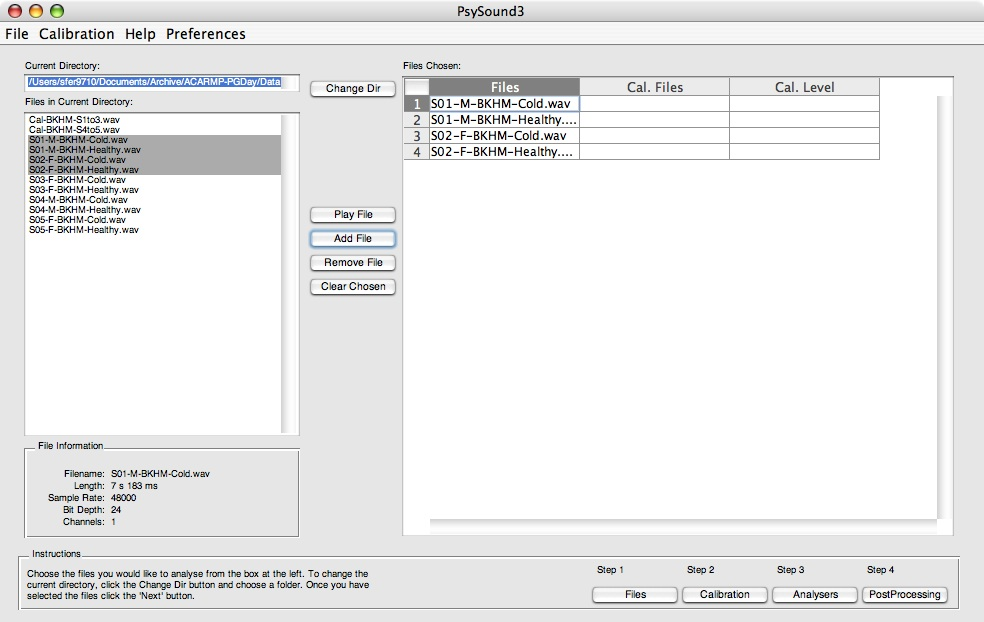
\includegraphics[width=3in]{Step1-AddingFiles.jpg}
	\caption{Choose files from the left column and then click `Add files' to add them to the list of files you have chosen to analyse.}
	\label{fig:stage01}
\end{figure}

You now can use the `Change Directory' button to choose this directory. PsySound will look at each file and find out a little information about each. It will then present you with all of the files in the box to your left.

You then need to add the files you wish to analyse. You can choose them and add them one by one, or you can select multiple files (with shift clicking, control clicking  or command clicking depending on platform) and add them all. You can remove files as well if you wish.

\subsection{Step 2 - File Calibration}

The next stage is to calibrate your files. Many of the audio analysis algorithms in the package behave differently depending on the sound pressure level the audio file represents. The way to control this is to change the sound pressure level of the file to make sure it is the same as the sound pressure level the microphone that recorded it received. This means that the algorithm will be receiving a sound pressure level that is appropriate for it to use. 

To do this we can either calibrate the microphone exactly, or estimate the sound pressure level that the microphone received. When we calibrate the microphone we record a known sound pressure level (from a specially calibrated sound source) and adjust the file until it exactly represents that known sound pressure level.

\begin{figure}[htbp]
	\centering
		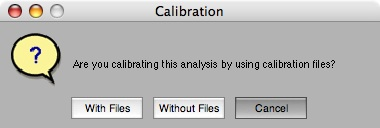
\includegraphics[width=3in]{Step2-ChoosingMethod.jpg}
	\caption{Choosing whether to calibrate with pre-recorded files, or to estimate the sound pressure level of the files to be analysed.}
	\label{fig:stage03}
\end{figure}

In PsySound3 these two methods are avilable, and you must choose between them when you begin the second stage. When you click on Step 2 you are asked to choose between calibration `With Files', and calibration `Without Files'. These two options represent the two possible ways of calibrating PsySound3 discussed above. 

If you choose the option `With Files' you will then be presented with a similar layout to the file selection you used in step 1, however, this time you will be associating calibration files with their respective audio files. It is common to calibrate the microphone at the beginning of the recording session and make multiple recordings in the session -- so it may be that you will have only one calibration file for a large set of recordings. However, the recording process involves many separate recording sessions then it is likely the microphone would be calibrated at the beginning of each recording session, and thus there may be a calibration file for each file to be analysed.

Each of the files to be analysed needs to be associated with its respective calibration file, and then the known sound pressure level that was recorded needs to be provided in each case. 

\begin{figure}[htbp]
	\centering
		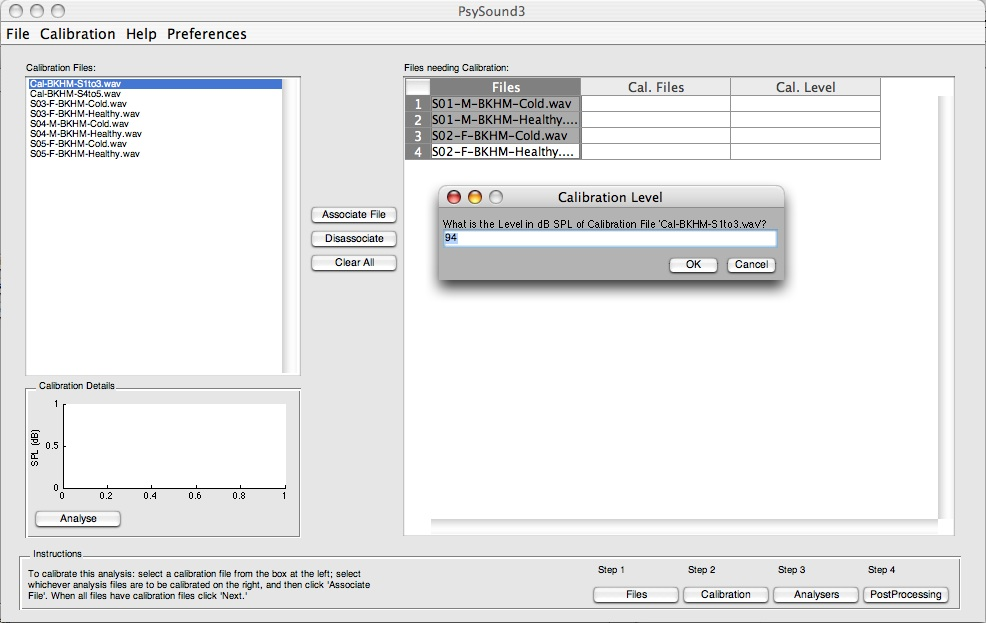
\includegraphics[width=3in]{Step2-SupplyLevel.jpg}
	\caption{Telling the program what sound pressure level the calibration files represent.}
	\label{fig:stage05}
\end{figure}

If you choose the second option, `Without Files' you will need to decide how you want to control the level of the files. There are a few options, you can:

\begin{itemize} 
\item Choose to change all the file's sound pressure levels to one specific  level -- this will mean comparisons are based on factors other than average level. In this case you will need to specify a level and a weighting scheme to use to calculate the level.
\item Choose to change all the file's sound pressure levels to the file with  either the greatest, the median, or the smallest sound pressure level.
\item Choose to make no change to the levels. 
\end{itemize}

\begin{figure}[htbp]
	\centering
		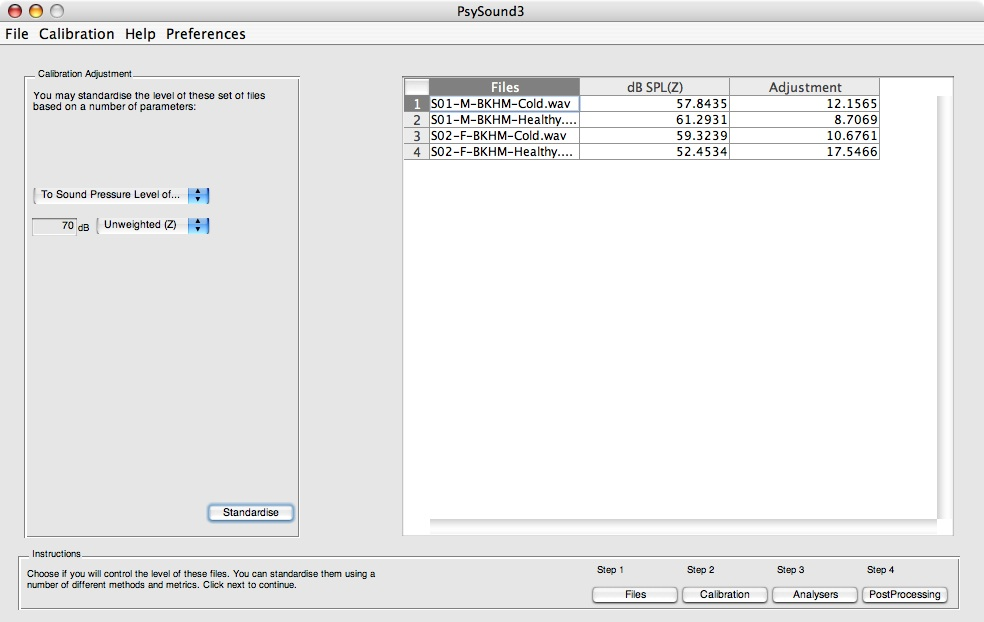
\includegraphics[width=3in]{Step2-StandardiseTo70.jpg}
	\caption{Standardising all files to 70dB, rather than providing recorded calibration files.}
	\label{fig:stage04b}
\end{figure}

Remember that if you change all the files to an average level (eg. 70dB) you then cannot compare the differences between sound pressure level and other similar algorithms, as these factors have been specifically controlled. Understanding calibration is essential, because if the wrong method is chosen then all results produced will be corrupted for some of the algorithms. Specifically, at least the the Terhardt Virtual Pitch algorithm, and all of the Loudness algorithms will be non-linearly affected by incorrect calibration - many of the other pitch and spectral analysers may only be linearly affected. Different procedures require different approaches to calibration, so there is no one method that can be recommended.

When a method is chosen and the standardise button is pressed, the program calculates the current average level (using the chosen weighting scheme) of each file, and the adjustment necessary to calibrate the file for use.

\subsection{Step 3 - Analysis with AudioAnalysers} 

AudioAnalysers are our name for the analysis modules that work with audio files in PsySound3. The available AudioAnalysers are presented to you in the box to your left in Step 3. 

\begin{figure}[htbp]
	\centering
		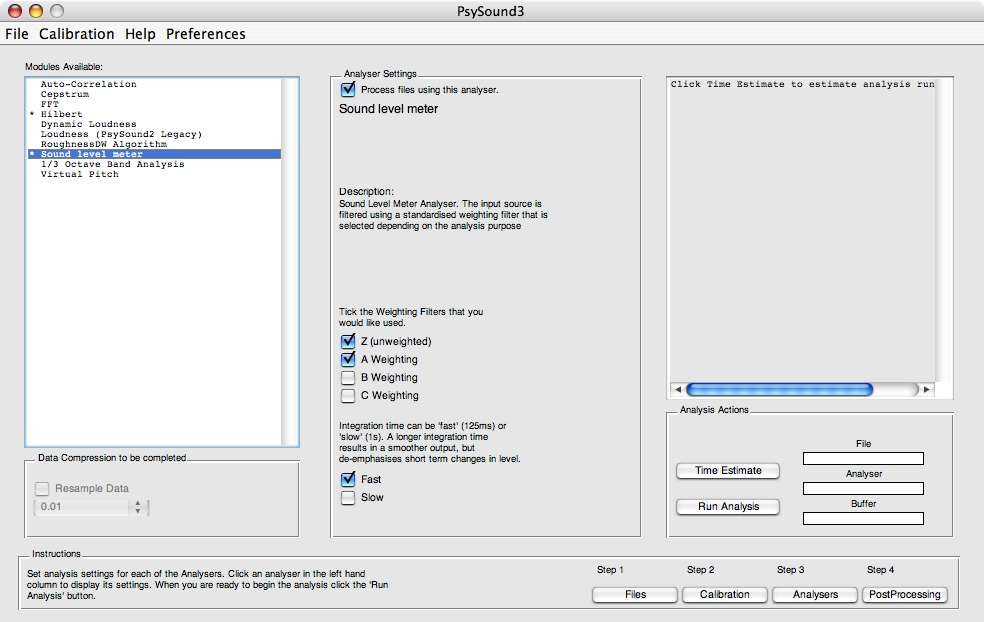
\includegraphics[width=3in]{Step3-ChooseAnalyser.jpg}
	\caption{Choosing an AudioAnalyser.}
	\label{fig:stage08}
\end{figure}

When you click on one of the AudioAnalysers you will be presented with a user interface for that AudioAnalyser, including the box you need to tick to enable that AudioAnalyser for this analysis session. Once you have selected the appropriate AudioAnalysers you will need to set the analysis going. 

You can click the `Time Estimate' button to get an estimate of how long it will take, and this may be useful as various AudioAnalysers will take different amounts of time depending on both their alogorithm's complexity, and the settings you have chosen to use. Finally when you are prepared to begin audio analysis you should click the `Run Analysis' button. The three progress bars will indicate the progress of the analysis process. When the analysis process is finished you will be moved on to Step 4, where you can see the results of your analysis.

\begin{figure}[htbp]
	\centering
		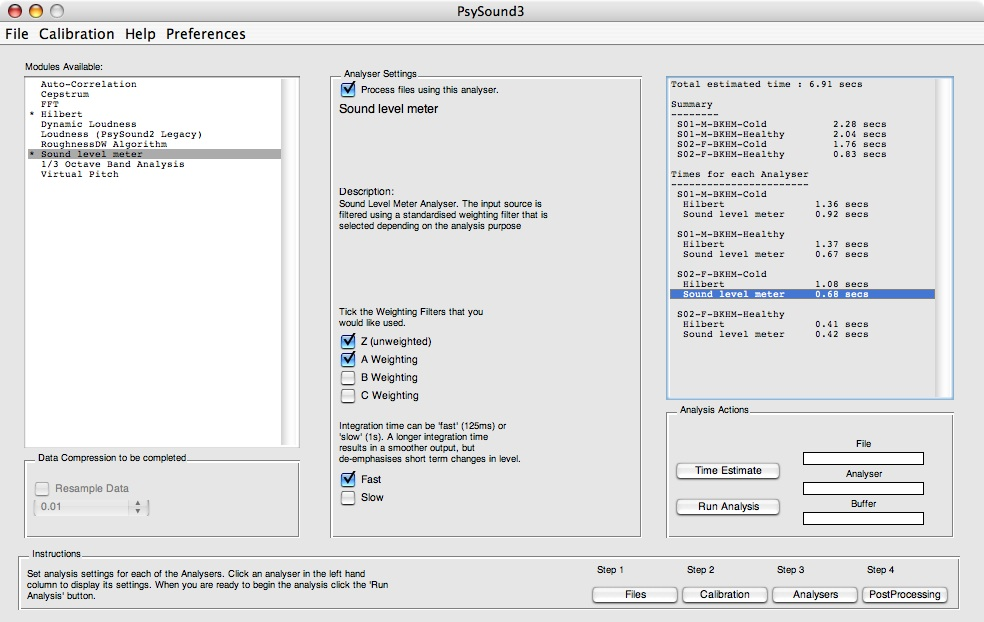
\includegraphics[width=3in]{Step3-TimeEstimate.jpg}
	\caption{Getting an estimate of how long it will take to process the files you have chosen to analyse.}
	\label{fig:stage10}
\end{figure}

For each audio file that is analysed there will be an AudioAnalyser result saved (on your hard drive), which will contain a set of various data objects that have been produced by the AudioAnalyser. 

There are three main types of data object used in PsySound3,
\begin{description}
 	\item[timeseries] data is data that involves one variable changing over time;
	\item[spectrum] data is a spectrum that represents the whole file; 
	\item[timespectrum] data is spectral data that changes over time;
\end{description}

\subsection{Step 4 - AudioAnalyser Output Analysis with DataAnalysers}

Once the audio analysis process is completed there will be an interface presented that allows you to apply various DataAnalysers to the data. These data analysers can consist of processes that allow you to graph, export or further transform and analyse the data in various ways. 

To begin with, open the tree node on on the left, and you will be shown the various files in the dataset. You can then progress to open the node that will show the AudioAnalysers that have been run on this file. You can then choose an AudioAnalyser result to work with and you will be shown the various data objects. You can then choose to further visualise or sonify the data objects you have chosen by choosing options from the tabs on the right. 

Each Data Analyser falls into one of the five categories, Visualisation, Sonification, Statistics, DataExport or DataAnalysis. There is also a summary page that shows you simple information about each file, Analyser or Data Object. 

When you click on each of the tabs a new DataAnalyser panel should open below. Between the tabs and the panel should be a popup menu which allows you to choose other DataAnalysers within that category. Usually the default DataAnalyser should be enough to begin with. Ideally buttons will be disabled unless you have selected the right combination of data objects to allow the command to be processed. For instance, the Multi-Graph button should only be available if two objects of the same type are selected.

\begin{figure}[htbp]
	\centering
		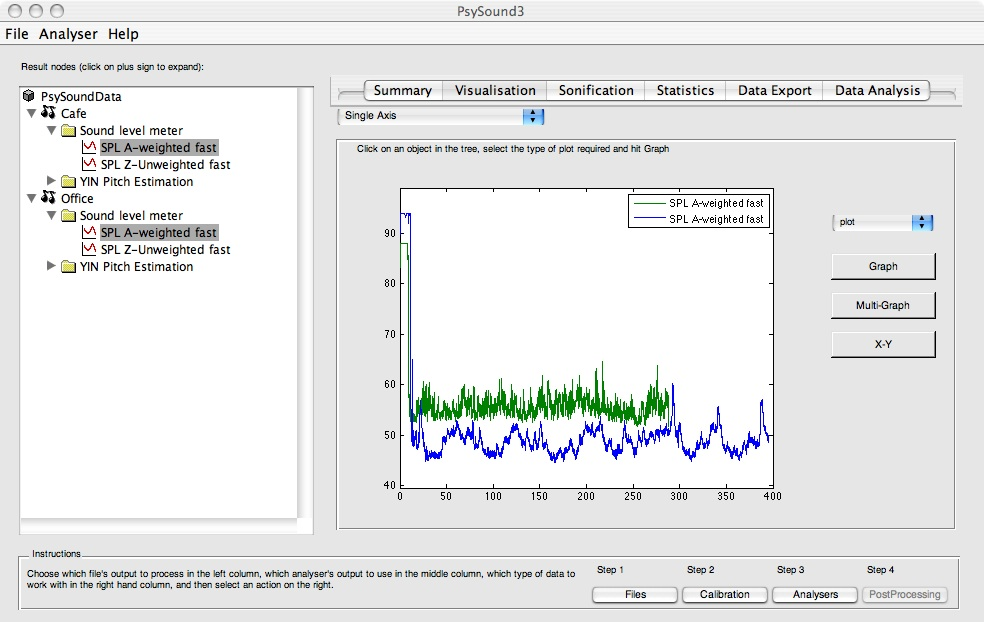
\includegraphics[width=3in]{Step4-NodeOpen.jpg}
	\caption{Choosing a timeseries data object and graphing it.}
	\label{fig:stage12}
\end{figure}

\clearpage
\section{Command Line Interface}

PsySound3 also has a command line interface that is useful for scripting analysis processes. It is used by the Graphical User Interface, and thus the algorithms and results are identical. 

The file-handling, windowing and overlapping reading is controlled by an function that creates a struct in the following way when a filename is passed to it:

\texttt{  >> fh = readData('BKHM-M-S03-MDV3-Student.wav')}

You will notice that there is a calCoeff field in the `fh' object. This needs to be set for the analysis to proceed. It is the multiplier which is applied to the data as each window is read, and therefore a good default value is 1. 

\texttt{ >> fh.calCoeff = 1;}

This creates a file handle which can then be used to instantiate the analysis objects. Each analysis object collects attributes of the file handle and configures itself for analysis with default parameters. Some of the analysis objects have further attributes that can be reconfigured if necessary. For instance if we were to use the Sound Level Meter analyser we would call:

\texttt{  >> obj = SLM(fh)}

The analysis process is controlled by the  method that needs to be called. The process method takes a first argument with the object, a second argument with the calibrated fileHandle and a final empty argument. This call is the same no matter which of the analysers you use.

\texttt{ >> obj = process(obj,fh,[])}

Once you have completed these steps you can look at the analyser output in the \texttt{obj.output} cell array. Inside this cell array will be data objects that you can work with further. For instance,\texttt{  plot(obj.output{1})} should give you a plot of the first data object. You could move these objects to separate variables for easier access: eg. \texttt{outData1 = obj.output{1};}. 

\subsection{Data Set Analysis Wrapper}

The above deals with specific commands to work with each of a number of analysers. There is also an interface to set up an analysis using a set of analysers and calibration files. This simplifies the process of working with multiple files and analysers. 

To create an array of file handles from a cell array of strings:

\texttt{fhs = readData({'file1.wav', 'file2.wav,', 'file3.wav'})}

To estimate the time the analysis will take 

\texttt{runanalysis(fhs, {'FFT', 'Hilbert', 'SLM'}, 'estimate')}

To calibrate your files by using a file `CalFile.wav' that represents 91 dB:

\texttt{fhs = calibrate(fhs, 'WithFiles', 'CalFile.wav', 91)}

or without files you specify the weighting (A, B ,C or Z) and the scheme (Max, Min)

\texttt{fhs = calibrate(fhs, 'WithOutFiles', 'A', 'Max')}

To run the analysis:

\texttt{objs = runanalysis(fhs, {'FFT', 'Hilbert', 'SLM'}, 'verbose')} 

and objs will be an array of data objects you can then work with.

\clearpage
\section{Writing New AudioAnalysers}

It is quite possible that the inbuilt audio analysers will not be appropriate for the feature detection task you wish to perform, or that you may wish to build in a feature detector of interest in order to compare it to the measures already in PsySound3. To cope with this possibility there is a simple interface for building new AudioAnalysers. 

Audio Analysers are defined here as analysis algorithms that are applied to audio signals. Thus they are logistically bound to the data source, and there are many commonalities between multiple Audio Analysers. Therefore we have defined in software a simple mechanism for adding Audio Analysers to the program. 

These Audio Analysers are known to the program as `classes', and your job is to add a new one. When the program is run, it looks at how many classes of the AudioAnalyser type there are available to it, and then it allows you to use them as you see fit. If you look in the program's code you will see that there is a directory called `Analysers', and within it there are a number of directories corresponding to each of the builtin AudioAnalysers. 

To add a new AudioAnalyser you will need a piece of audio analysis code (an m-file function usually) you wish to add. It should take as an input a short window of sound (usually something like 128-8192 samples long), and output some other type of data. The process for making this piece of code into a new class is to take an empty AudioAnalyser and modify 4 files in order to `wrap' this piece of code.  

It is easier to understand what you need to modify if we first look at what the program does with each Audio Analyser. Whenever it is asked to analyse a file, it makes a reference to the file, sends that reference to an AudioAnalyser (which may or may not need a few more settings) and then calls the `process' command for that AudioAnalyser. The process command starts the process described in Figure 	\ref{fig:AADiagram}

\begin{figure}[htbp]
	\centering
		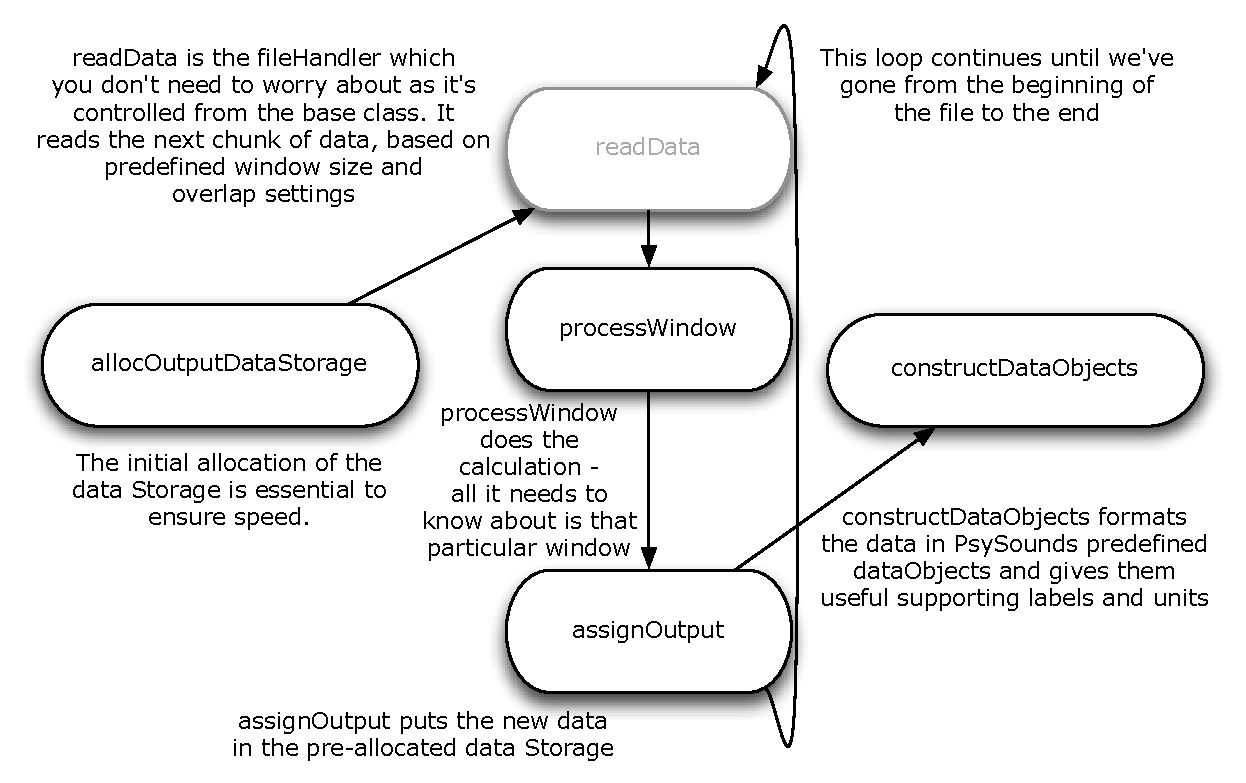
\includegraphics[height=3in]{AudioAnalysersDiagram.pdf}
	\caption{The `process' command initiates the AudioAnalyser's process of analysing the audio data.}
	\label{fig:AADiagram}
\end{figure}

That process is to:

\begin{description}
	
\item[allocOutputDataStorage.m] Allocate matrices for assigning the data, so that the program can neatly slot the appropriate data into the appropriate slot, whenever each calculation is finished. The size of the data buffers is calculated based on the length of the file to be analysed and the appropriate settings, including the overlap and the window length. 

\item[readData.m] Read a chunk of the data. Which chunk is read is controlled by the overlap setting, and a window is applied based on the settings chosen. (This file does not need to be altered when adding an AudioAnalyser.)

\item[processWindow.m] Process the window. This is the file that actually does the calculations, and it needs to return some kind of data. This is usually a very small file, just consisting of the necessary call to whichever calculation function is to be used. 

\item[assignOutputs.m] This takes the result of processWindow.m and places it in the data buffers that have been allocated in allocOutputDataStorage.m. 

\emph{These 3 files (readData, processWindow and assignOutputs) are a loop that is repeated until the entire file is read.}

\item[constructDataObjects.m] THe data buffers are now completely full, and thus they can be reformatted into appropriate PsySound data objects, replete with axis names and units. There are three main data Objects they are formatted to: the Spectrum object, the Timeseries object, and the Timespectrum object.

\end{description}

In addition to these methods, used whilst the file is being processed, there is also the AudioAnalyser constructor that needs to be altered. 

\subsection{Step By Step How-to}

Following are step by step instructions to making your code into an analyser. These assume you have unzipped the TemplateAnalyser folder into the `Analysers' folder, and that you have a piece of code called `mycode.m' that you wish to wrap. Lets assume you will call your new Analyser  `myAnalyser'. We are not going to deal with extra features like customised user interfaces or control of windowing settings in this particular how-to. 

\subsection{TemplateAnalyser.m}

\begin{itemize}
	\item Rename the folder `@TemplateAnalyser' `@myAnalyser'. You need the @ symbol to be at the front.  
	\item Inside that folder rename the file `TemplateAnalyser.m' to `myAnalyser.m'. 
	\item Inside the file myAnalyser.m change the references to `TemplateAnalyser' to `myAnalyser'.
\end{itemize}

\subsection{allocOutputDataStorage.m}

To work out which data buffers to allocate you need to think about what your algorithm puts out. Many algorithms return a single number for each window  processed. Others transform the input data in some way, and therefore often end up with the same amount of data coming out as goes in. 

To work out how many windows there will be for this particular file use \texttt{getNumWindows(obj)}. If, say, your algorithm returns only one number per window analysed, then you simply need to make a data buffer for that number of windows:

\begin{verbatim}
pts               = getNumWindows(obj); 
dataBuffer.myData = makeDataBuffer(pts, 1);
\end{verbatim}

\texttt{allocOutputDataStorage.m} returns only \texttt{dataBuffer} and therefore you need to attach your new dataBuffers as fields of this `struct'. The code above creates a matrix that is `pts' long and only 1 cell wide, basically a big list.

If your file actually returns one quarter of the size of the window analysed, then you need to set up a matrix for the data buffer. This will require knowing the size of the window (as it can often be changed). 

\begin{verbatim}
pts               = getNumWindows(obj);
windowLength      = get(obj, 'windowLength'); 
dataBuffer.mySpecData = makeDataBuffer(pts, windowLength/4);
\end{verbatim}

The code above creates a matrix that is `pts' long and `windowLength/4' cells wide, which allows the storage of spectra that change over time.

You should attach as many dataBuffers as you will need.

\subsection{processWindow.m}

processWindow.m is usually very simple - it just calls the myCode file. Its argument is `dataIn', and its output is dataOut. Therefore as our function is called \texttt{mycode.m}:

\begin{verbatim}
dataOut = mycode(datain);
\end{verbatim}

should do it for us. 

\subsection{assignOutput.m}

\texttt{assignOutput.m} simply works to take the \texttt{dataOut} data that we have seen before and plonk it in the data buffer at the appropriate index. It has a lot of arguments:

\begin{verbatim}
	obj = assignOutputs(obj, dataIn, index, dataBuffer, s)
\end{verbatim}

Again you can get useful information about the `obj' by using the get method, and you can alter and format the data to a certain extent before it is stored.  But the most important method, the `assign' method, is a function handle attached to the \texttt{dataBuffer} object. This assigns the data taken from the processWindow.m file to the dataBuffer. Therefore

\begin{verbatim}
dataBuffer.myData.assign(index, dataIn, 'row');
 \end{verbatim}

will assign the \texttt{dataIn} to the current \texttt{index} in the \texttt{myData} buffer in the collection of buffers called \texttt{dataBuffer}.

\subsection{constructDataObjects.m}

Finally, once the process is finished we send the collection of dataBuffers to the constructDataObjects file for formatting into data Objects. We have 3 dataObjects for storing data.  

\begin{description}
	\item[tSeries] is a format for saving time series data in, it is a customised form of the builtin matlab timeseries objects. 
	
	\item[Spectrum] is used to save Spectral data that does not have a time axis.
	
	\item[tSpectrum] is used for saving spectral data that varies over time. It's commonly stores much biger sets of data.
	
\end{description}
	 
Fundamentally we need to get the data from the dataBuffer and create a dataObject that matches its type. We call the \texttt{createDataObject} function, and pass it the type of dataObject to make, the data, and a vector that represents the frequency and time data that will be used with it. 

Once these files are filled in the process will automatically be picked up by the program


\subsection{Raw Interface}

The above method for writing Audio Analysers requires a fair amount of knowledge of the internal workings of PsySound3, and is used in many of the algorithms supplied. However, recently we have been experimenting with a simpler method for processing files - based on providing the entire analysis file data, using one call to the underlying analysis code which usually can be left completely untouched. More information on this method can be found by investigating the SWIPEP analyser. This will eventually become the standard method for developing analysers. 


\clearpage
\section{Writing New DataAnalysers}

There are various ways of analysing the data that is produced by the AudioAnalysers. These methods of analysis we have called DataAnalysers, and they are another user-definable part of PsySound3. There is number of examples of DataAnalysers which are distributed with the program, but the real power is the possibility to write your own.

These methods work on the data objects we have defined -- as they are standardised it is possible to define analysis methods without knowing which AudioAnalyser's output the method will be applied to. As long as the output data is in a standard format the DataAnalyser should be able to work with it.

This is a simpler process, and requires you to:

\begin{itemize}
	\item write a user interface to the process
	\item load in the selected data objects
	\item process or act on the data objects in some way
	\item display or save the result
\end{itemize}

We have categorized the possible DataAnalysers into four general fields: 
\begin{description}
\item[Visualisation:] the visual representation of data;
\item[Sonification:] the representation of data through sound;
\item[Statistical Analysis:] Statistical methods for transforming data; 
\item[Data Export:] Export of raw data in various formats.
\end{description}

Within each of these general categories there is a number of DataAnalysers that perform specific purposes. Each Data Analyser can be chosen from the pulldown menu below the list of tabs. 

If we look at the BasicPlot DataAnalyser (available to read in the DataAnalysers folder) we  can see most of the important files you will need to define to build a DataAnalyser. They will be dealt with one by one in the following How-To. We will assume you wish to write an analyser called `ComplexPlot', and that it will be in the Visualisation category. 

\subsection{Folder: @BasicPlot}

The folder that contains all the code for the BasicPlot DataAnalyser is called  `@BasicPlot'. We need to create a new folder called `@ComplexPlot' for our new set of code. The `@' is necessary for the DataAnalyser to be understood by Matlab. All further code mentioned should be placed inside this new folder. 

\subsection{Constructor: BasicPlot.m}

The constructor can be copied completely for your new DataAnalyser. There are only a couple of parts to change. Obviously the name of the DataAnalyser is set in this file, so it is necessary to change it here. Wherever there is a `BasicPlot' it will be necessary to change it to `ComplexPlot'. This includes the filename \texttt{BasicPlot.m}. 

The category of the Data Analyser can be set by changing the line that reads: 

\texttt{obj = set(obj, 'Group', 'Visualisation');}

`Visualisation' can be one of the four categories listed above -- Visualisation, Sonification, Statistical Analysis, Data Export.  


The name of the Data Analyser that appears in the popup menu below the tabs can be set by changing the line that reads: 

\texttt{obj = set(obj, 'Name',  'Single Axis');}

to whatever name you would like the DataAnalyser to display.

\subsection{User Interface: ui.m}

The user interface is built inside the panel to the right of the data output selection tree. The panel's handle is passed to the ui.m file, and user controls can be built on the panel in the usual manner for building user interfaces in Matlab. Each of the user interface controls that are built should have a unique `Tag' field, as these are used later to get the choices that the user has made. 

For information about user interface elements check the Matlab help for \texttt{uicontrol}. The `GUIDE' method in Matlab is an automated system that is not helpful in this particular case.

\subsection{User Interface: updateDataAnalyserPanel.m}

Sometimes when users make particular choices it is appropriate to change the user interface in various ways. The most obvious example is a DataAnalyser user interface that turns buttons on or off when different data objects are chosen in the output data tree. This can be achieved by using the \texttt{updateDataAnalyserPanel.m} file, and altering the Enable field of the user interface elements you have employed. 

In the BasicPlot example the \texttt{updateDataAnalyserPanel.m} file is used to turn on and off different buttons, depending on how many data objects are chosen. It finds each of the user interface elements by their `Tag', and then alters the `Enable' field to grey them out if they are not useful with this particular number of selected objects, or make them active if they are.

This stage is completely optional, but can be very useful for making a more usable user interface. 

\subsection{Callback: Graph.m}

The \texttt{Graph.m} file contains the code that performs the actual graphing for BasicPlot. 

The main methods that are essential are that the user choices are found by accessing the user interface elements by their `Tag' again. For instance:

\texttt{plotPopup = findobj(p, 'Style', 'Popup', 'Tag', 'PlotTypePopup');}

is used to find the popupmenu based on its unique Tag `PlotTypePopup'. They then find the choices by looking at the fields in the user interface elements. For instance:

\texttt{plotStrs  = get(plotPopup, 'String');}

There are built-in methods for finding which of the data objects from the output data tree have been selected: 

\texttt{nodes = getSelectedTreeNodes(obj, p);}

This will produce an array of names that can then be loaded specifically thus: 

\textt{dataObj = getDataObjectFromTreeNode(obj, nodes(1))}

In this case, dataObj is the first node from the the array of selected data Objects.

Inside the dataObj struct there are two fields, DataObj and AnalyserObj. AnalyserObj contains information about the analyser's settings when the analysis was performed. This is useful for finding the settings of the window,the sample rate or the filename. The DataObj field contains the dataObject that is used for the actual processing. 
 
The fields of the data object contain the actual data, as well as axis information and unit names. This data can be used for the data analysis process directly.  As an example, the BasicPlot code listed below plots two time series data sets against each other using an X-Y Scatterplot. This assumes that the data is equally sized, and that there are no problems loading the data from the `nodes' array we have previously retrieved.  

\begin{verbatim} 
	dataObjS = getDataObjectFromTreeNode(obj, nodes(1));  
	dataObj1 = dataObjS.DataObj;
	data1    = dataObj1.Data;
	dataObjS = getDataObjectFromTreeNode(obj, nodes(2));
	dataObj2 = dataObjS.DataObj;
	data2    = dataObj2.Data;
	plot(data1, data2);
	xlabel(dataObj1.DataInfo.Units);
	ylabel(dataObj2.DataInfo.Units);
	title([dataObj2.Name, ' vs ', sprintf('\n'), dataObj1.Name]);
\end{verbatim}

There are many more methods available to use, and many of the included  DataAnalysers demonstrate their usage. This document has served to explain the fundamentals of DataAnalysers, but the best way to learn is to look through the DataAnalysers distributed with PsySound3, and work out how they work. The methods in the base class directory (@DataAnalyser) are also of relevance.

\end{document}   

